\chapter{Background}
\label{chapter:background}

This chapter presents a literature review of various optimization concepts
relevant to the analysis of Hash Code problems as well as the framework detailed
in ~\cite{outeiro2021application}, which will be used and potentially improved upon throughout
this work. Additionally, it provides background on essential concepts such as modelling
and meta-heuristics, which will be further discussed in subsequent chapters.
In particular, Section~\ref{section:optimization-concepts}~presents a series
of combinatorial optimization concepts relevant to this work, whilst
Section~\ref{section:meta-heuristics}, delves into the definition of meta-heuristics
and provides key concepts and examples. Finally, Section ~\ref{section:modelling} presents
the concept of modelling and offers insight into current frameworks and
API~\cite{outeiro2021application,vieira2009uma} based around this idea.

\section{Optimization Concepts}
\label{section:optimization-concepts}

Optimization involves finding the best solution to a given problem among a set
of feasible solutions. Specifically, considering the single objective case
involves finding the optimal configuration or set of parameters that maximize or
minimize an objective function, possibly subject to constraints on its
variables~\cite{nocedal2006numerical}.Given that, and as defined by
Papadimitriou and Steiglitz~\cite{papadimitriou1998combinatorial}, an
optimization problem can formally be described as follows:

\begin{definition}[Optimization Problem~\cite{papadimitriou1998combinatorial}]
    \label{def:optimization-problem}
    An optimization problem is a collection $\mathcal{I}$ of instances,
    typically generated in a similar manner. An instance $\iota$ of an
    optimization problem consists of a pair $(\mathcal{S}, f)$, where
    $\mathcal{S}$ is a set containing all feasible solutions, and $f$ is an
    objective (cost) function, with a mapping such that:
    \begin{equation}
        \label{equation:optimization-problem}
        f \colon \mathcal{S} \longrightarrow \mathbb{R}
    \end{equation}
    That is, for each solution $s \in \mathcal{S}$, a real value is assigned to
    indicate the quality of the solution. Thus, the problem consists in finding
    a global optimal solution $s^* \in \mathcal{S}$, for each instance $\iota$.
\end{definition}

\begin{definition}[Global Optimal Solution~\cite{hiriart-urruty1995conditions,papadimitriou1998combinatorial}]
    \label{definition:global-optimum}
    Assuming, without loss of generality, an optimization problem with a
    maximizing objective function $f(s)$, a global optimal solution $s^*$ is
    expressed by:
    \begin{equation}
        \forall s \in \mathcal{S} \colon f(s^{*}) \geq f(s)
    \end{equation}
\end{definition}

Given that the Hash Code problems are designed with a maximizing objective
function, only maximization problems will be considered in this work.
Nonetheless, a minimizing objective function $f(s)$ can be reformulated for
maximization by using the identity \textit{$\max{-f(s)} = \min{f(s)}$}.

\subsection{Combinatorial Optimization}
\label{section:combinatorial-optimization}

There are two main categories of optimization problems based on the domain
of the variables: discrete and continuous. In problems with discrete variables,
the solutions are defined on a finite, or countably infinite, set of values. In
contrast, for problems with continuous variables, the solutions take on any
value on a continuous (infinite) subset of real numbers. Nonetheless, there
are also problems that involve both categories commonly denominated as
mixed~\cite{nocedal2006numerical}.

\begin{definition}[Combinatorial Optimization Problem~\cite{papadimitriou1998combinatorial}]
    \label{def:combinatorial-optimization-problem}
    An instance $\iota$ of a combinatorial optimization problem is an instance of an
    optimization problem (\ref{def:optimization-problem}) where the set
    $\mathcal{S}$ of feasible solutions is finite or countable infinite.
\end{definition}

\acrfull{combinatorial-optimization} problems~\ref{def:combinatorial-optimization-problem}
are a subset of discrete optimization problems characterized by a discrete
solution space that typically involves different permutations, groupings, or orderings
of objects that satisfy certain criteria~\cite{vieira2009uma,papadimitriou1998combinatorial}.
As such, solutions for these problems are discrete objects related to the combinatorics e.g
integers, permutations sets and graphs.~\cite{blummetaheuristics,yu2010combinatorial}

Typical examples of \acrshort{combinatorial-optimization} problems include
network flow, matching, scheduling, shortest path and decision problems. Some
representative examples of such problems are the
\acrfull{travelling-salesman-problem} and the
\acrfull{knapsack-problem}~\cite{yu2010combinatorial}. In the case of
the~\acrshort{knapsack-problem}, given a set of items, each with a given weight
and profit, and a knapsack with a given maximum weight capacity, the goal is to
find the subset of items with the highest total profit that can be placed in the
knapsack without exceeding its capacity. As for the~\acrshort{knapsack-problem},
the goal is to find the shortest possible route that visits each city exactly
once whilst returning to the starting city i.e an Hamiltonian cycle.

\begin{definition}[Ground Set~\cite{outeiro2021application}]
    \label{definition:ground-set}
    The ground set $\mathcal{G}$ is a finite set of elements that represents all
    possible components that may integrate a feasible solution for a given
    instance $\iota$ of a CO problem.
    \begin{equation}
        \label{equation:ground-set}
        \mathcal{G} \colon \{c_{1}, c_{2}, c_{3}, \ldots, c_{i}\}
    \end{equation}
    Thus, a feasible solution is a subset of the ground set, denoted as $s \in
        \mathcal{S} \subseteq 2^{\mathcal{G}}$, and which may be encoded as a binary
    string indicating the presence (1) or absence (0) of a given component
    $c_{i}$.
\end{definition}

Given the discreteness of the decision space in \acrshort{combinatorial-optimization}
problems, the solutions are constructed by combining objects present in a finite set
containing all the individual components that fully characterize a solution.
This set, commonly denominated ``ground set''
\cite{outeiro2021application,festa2014brief,marti2013multistart}, can be defined
as shown in~\ref{definition:ground-set}:

Regarding the definition of a \acrshort{combinatorial-optimization} problem
\ref{def:combinatorial-optimization-problem} and alluding to the solution
representation as a binary string, we can then define both the feasible solution
set $\mathcal{S}$ and the ground set $\mathcal{G}$ for the \acrshort{knapsack-problem}
and the \acrshort{travelling-salesman-problem}.

\begin{itemize}
    \item \textbf{\acrlong{knapsack-problem}}: The set of feasible
          solutions $\mathcal{S}$ consists of all possible subsets of items that can
          be placed in the knapsack without exceeding its weight capacity. The ground
          set $\mathcal{G}$ is a set of all possible items that may be included in a
          feasible solution~\cite{festa2014brief}. As such, a solution $s \in
              \mathcal{S}$ can be represented as a binary string, where the $i^th$
          position of the string contains a value of 1 or 0 depending on whether the
          $i^th$ item in $\mathcal{G}$ is present or absent in the final solution.

    \item \textbf{\acrlong{travelling-salesman-problem}}: The set
          $\mathcal{S}$ consists of all possible Hamiltonian cycles representing the
          order in which cities should be visited, typically represented as a
          permutation. The ground set $\mathcal{G}$ in this case can be thought of as
          a set containing all possible paths between two distinct cities, i.e. edges
          in a graph~\cite{marti2013multistart,festa2014brief}. Hence, a solution $s
              \in \mathcal{S}$ can be represented as a binary string where the $i^{th}$
          position of the string contains a value of 0 or 1 depending on whether a
          given edge connecting two cities is present or absent in the final solution.
\end{itemize}

In summary, since \acrshort{combinatorial-optimization} problems involve
choosing a combination of objects any algorithm that is able to enumerate the
entirety of the solution space can be used to solve these problems. However, finding optimal
solutions can be difficult, and exhaustive search strategies may not be able to
solve many of these problems, which are often
NP-Hard~\cite{yu2010combinatorial,festa2014brief} and thus not approachable by
algorithms in a reasonable amount of time. In these cases, approximation or
heuristic/meta-heuristic methods present themselves as effective alternatives to be considered.

\subsection{Global and Local Optimization}

With regard to the search of solutions for optimization problems, there are two
primary strategies: \acrfull{global-optimization} and
\acrfull{local-optimization}.

\acrshort{global-optimization} refers to the process of identifying a global
optimal solution (\ref{definition:global-optimum}) to a given problem,
regardless of its location within the solution space. In contrast,
\acrshort{local-optimization} focuses on finding the best solution among those
that are proximate in some sense. The concept of proximity is related to the
definition of a neighborhood, which for a given solution is specified by a
particular neighborhood structure defined as follows:

\begin{definition}[Neighborhood Structure~\cite{papadimitriou1998combinatorial, blummetaheuristics}]
    \label{definition:neighborhood-structure}
    A neighborhood structure for an optimization problem with instances $(\mathcal{S}, f)$ is a mapping:
    \begin{equation}
        \label{equation:neighborhood-structure}
        \mathcal{N} \colon \mathcal{S} \longrightarrow 2^{\mathcal{S}}
    \end{equation}
    Such that, a set of neighboring solutions $\mathcal{N}(\hat{s}) \subseteq
        \mathcal{S}$ is assigned for each solution $\hat{s} \in \mathcal{S}$.
    This referred to as the neighborhood of $\hat{s}$.
\end{definition}

In general, the neighborhood structure refers to the set of rules that
must be applied to a solution in order to generate all of its neighbors.
Additionally, we consider the following definition of local optimal solution.

\begin{definition}[(Strictly) Local Optimal Solution~\cite{blummetaheuristics,nocedal2006numerical}]
    \label{definition:local-optimum}
    Assuming maximization without loss of generality, a solution $\hat{s}$ is
    local optimal with respect to a given neighborhood structure $N(\hat{s})$
    iff:
    \begin{equation}
        \label{equation:local-maximum}
        \forall s \in \mathcal{N}(\hat{s}) \colon f(\hat{s}) \geq f(s)
    \end{equation}
    Furthermore, $\hat{s}$ is considered strictly global optimal iff
    \begin{equation}
        \label{equation:strict-local-maximum}
        \forall s \in \mathcal{N}(\hat{s}) \setminus \{\hat{s}\} \colon f(\hat{s}) > f(s)
    \end{equation}
\end{definition}

As an illustrative example, consider the objective function $f(s)$ shown in
figure~\ref{fig:maxima}. With respect to the definitions~\ref{definition:global-optimum}
and~\ref{definition:local-optimum} $s^2$, $s^3$ are (strictly) local optimal.

\begin{figure}[h]
    \centering
    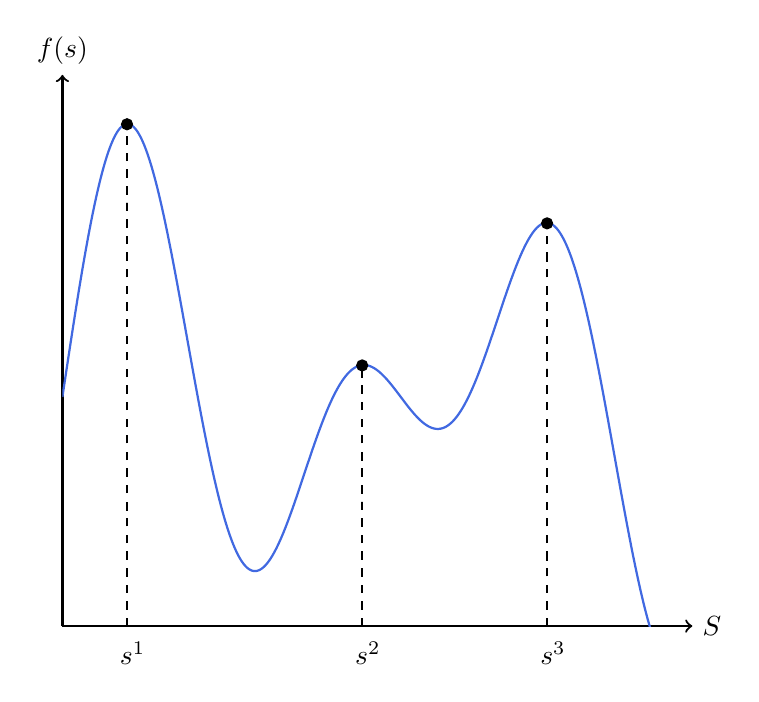
\begin{tikzpicture}
	% Axis Lines
	\draw[->, thick] (0,0) -- (8,0) node[right] {$S$};
	\draw[->, thick] (0,0) -- (0,7) node[above] {$f(s)$};

	\begin{axis}[axis lines = none,scale only axis=true,xmin=0,
			xmax=18.5,ymin=0,ymax=10]

		% Main Plot
		\addplot[domain=0:17,samples=1000,smooth,color=RoyalBlue,
			thick] {2.5*sin(deg(x)) + 2.5*sin(deg((2/3)*x)) + 4};

		% Vertical Line (s1)
		\addplot[domain=0:17,thick,samples=1000,dashed,
			smooth] coordinates {(1.8,0) (1.8,8.76)};
		\addplot[domain=0:17,mark=*] coordinates {(1.8,8.76)};
		% \draw (1.8,8.76) circle[radius=1.5pt];
		% \fill (1.8,8.76) circle[radius=1.5pt];

		% Vertical Line (s2)
		\addplot[domain=0:17,thick,samples=1000,dashed,
			smooth] coordinates {(8.35,0) (8.35,4.55)};
		% \draw (8.35,4.55) circle[radius=1.5pt];
		% \fill (8.35,4.55) circle[radius=1.5pt];
		\addplot[domain=0:17,mark=*] coordinates {(8.35,4.55)};

		% Vertical Line (s3)
		\addplot[domain=0:17,thick,samples=1000,dashed,
			smooth] coordinates {(13.5,0) (13.5,7.03)};
		% \draw (13.5,7.03) circle[radius=1.5pt];
		% \fill (13.5,7.03) circle[radius=1.5pt];
		\addplot[domain=0:17,mark=*] coordinates {(13.5,7.03)};
	\end{axis}

	% Labels
	\node (s1) at (0.89,-0.35) {$s^1$};
	\node (s1) at (3.88,-0.35) {$s^2$};
	\node (s1) at (6.23,-0.35) {$s^3$};

\end{tikzpicture}


    \caption{Global and Local Optimal Solutions}
    \label{fig:maxima}
\end{figure}

In practice, the decision to use either a global or local optimization strategy
is often influenced by factors such as the available time budget and the
preferences of the decision maker. While global optimization aims to find the
optimal solution to a problem, the search process may be time-consuming or, in
some cases, computationally infeasible due to the size of the search space.
On the other hand, local optimization, while lacking the optimality guarantees
of global optimization, is able to quickly generate good solutions that may
be acceptable to the decision maker. Nonetheless, the quality of the solutions
may be poor due to the ruggedness of the objective function fitness landscape
(many local optima). Ultimately, the performance of both methods is closely
tied to the knowledge of problem-specific features.

In a setting such as the Hash Code competition, the problems presented are
designed to resemble real-world situations. Additionally, due to the time
constraints, it is not in the interest of the contestants to use global optimization
methods, as they are unlikely to finish on more complex problem instances.
Instead, a balance between global and local optimization is typically employed,
with contestants utilizing the advantages of both methods. This approach
involves establishing a baseline with global optimization methods that explore
unseen regions of the search space for potentially good solutions, and then
utilizing local optimization methods for exploiting solutions that have
already been found.

\subsection{Black-Box and Glass-Box Optimization}

In the field of optimization, two settings are commonly recognized:
\acrfull{black-box-optimization} and \acrfull{glass-box-optimization}.

In \acrshort{black-box-optimization} optimization settings there is no
information about the landscape of the function being optimized, constraints
defining the set of feasible solutions~\cite{alarie2021two} or the objective function
is too complex to be approached from an analytical perspective. As such,
algorithms for achieving solutions for these problems do so only by interacting
with the problem through the evaluation of potential candidate
solutions~\cite{doerr2020complexity}. Meta-Heuristics, as will be later detailed
are examples of methods that follow this approach for finding/improving
solutions. By contrast, in \acrfull{glass-box-optimization} optimization, also
known as ``white box'' optimization, there is a good understanding of the
problem instance being optimized and the objective function
properties~\cite{doerr2020complexity}. Hence, the algorithms used may take
advantage of more analytical properties of the problem since they are
transparent to the optimizer.

For the purpose of clarification, with regard to the previously mentioned
\acrshort{travelling-salesman-problem}, a black-box strategy would entail the
utilization of a search heuristic such as simulated
annealing~\cite{luke2013essentialsa} to obtain solutions. This is because the
algorithm only necessitates knowledge of how to evaluate the quality of
solutions through the objective function and not any specific information about
the function being optimized. Alternatively, if the problem were to be
formulated as an Integer Linear Programming
problem~\cite{nocedal2006numerical,papadimitriou1998combinatorial}, it would
become amenable to a white-box approach, as the objective function would be
accessible, and additional information about the problem could be inferred from
it and provided to the algorithm.

In the context of the Hash Code competition, contestants typically engage with a
problem from a black-box perspective, as the underlying objective function of
the problem is not disclosed, and/or is too complex to formalize. Additionally,
the process of formalization would be time-consuming and, as a result, the usage
of white-box methods post-formalization would not be justified, given that they
may be computationally slower. Despite this, it is important to note that
white-box methods should not be overlooked as they construct a model of the
problem in order to solve it, which could be applied to a certain extent in the
context of black-box approaches.

\section{Optimization Strategies}
\label{section:optimization-strategies}

In the field of optimization, a vast array of algorithms have been extensively
documented in the literature for resolving various types of problems. These
algorithms can be broadly classified based on their time complexity, the
strategy employed to discover solutions, and the quality of solutions obtained.
Specifically, algorithms can be classified into three categories, based on
optimality of the solution found as exact, approximate, or heuristic. Moreover,
there are also general techniques for finding solutions, such as constructive
and local search methods. Additionally, the concept of bounds, which serve to
guide the search for solutions, is also a crucial factor that can be considered
as a strategy to enhance the optimization process.

\subsection{Exact, Approximation and Heuristic Approaches}
\label{section:approaches}

Exact approaches are techniques that aim to find the optimal solution for a
given problem. These approaches typically involve an exhaustive enumeration and
evaluation of solutions belonging to the set $\mathcal{S}$ of feasible solutions.
However, in complex real-world problem instances, this may prove to be
computationally infeasible. In the context of combinatorial optimization
problems, two general exhaustive search strategies are well-known and widely
studied: Branch and Bound and Dynamic Programming. These strategies work by
successively dividing the problem into smaller dependent or independent
sub-problems, and then combining the solutions to these sub-problems to obtain the
final solution.

Approximation approaches, in contrast, aim to find solutions that have a
guarantee on the quality of the feasible solution being close to the quality of
optimal solutions, within an approximation factor $\varepsilon$. Despite these
approaches often solving problems in polynomial time and yielding solutions of
relatively high quality, it is important to note that they require a
mathematical proof of approximation that is specific to the problem at hand.
There exists a significant amount of research in this field, particularly for
combinatorial optimization problems~\cite{johnson1974approximation}.

Lastly, heuristic approaches work by finding solutions according to a general
rule of thumb, the quality of which can be verified through experimentation.
These methods do not provide any guarantees of optimality, as they are derived
from intuition and their effectiveness is closely tied to the characteristics of
the problem at hand. Nevertheless, they are reliable means of finding solutions
in difficult combinatorial optimization (CO) problems. A well-known class of
algorithms that utilize this approach are meta-heuristics, as will be further
discussed in this work, with examples such as Greedy Randomized Adaptive Search
Procedures (GRASP), Simulated Annealing (SA) and Iterated Local Search (ILS).

\subsection{Constructive Search}
\label{section:contructive-search}

Constructive search (CS) is a procedure for optimization where from an empty or
partially complete solution for a given problem instance a feasible complete
solution is constructed by iteratively adding components extracted from the
ground set. The construction process is guided by a pre-established set of
rules, which may be heuristic in nature or informed by other relevant
information. These rules determine, at each iteration, the set of components
that are eligible for inclusion in the final solution.

CS approaches, as such, require certain information about the representation of
solutions and specifically, how the addition or removal of a given component or
set of components affects the overall quality of the solution, as measured by
the objective function value or other metrics such as bounds or dominance
relationships between solutions. It is crucial to note that the availability of
information about the problem at hand directly impacts the capability of these
strategies to optimize.

As an illustrative example, consider the aforementioned \acrshort{knapsack-problem} and
\acrshort{travelling-salesman-problem} from section
~\ref{section:combinatorial-optimization}. In this scenario, an example of a
constructive approach for the KP could involve selecting, in each step, the item
with the highest ratio of profit to weight that does not exceed the weight
capacity of the knapsack. Similarly, for the TSP, a constructive approach would
involve selecting an edge to add to the tour that contributes the most, while
ensuring that the primary constraint of constructing a Hamiltonian cycle is not
violated.

\subsection{Local Search}
\label{section:local-search}

In contrast to constructive search, local search (LS) procedures begin with a
feasible solution to a given problem instance, and then make small modifications
to its components by applying transformations, such as adding or removing
elements. These transformations aim to improve the solution within the
neighborhood, as defined by the problem's neighborhood
structure~\ref{definition:neighborhood-structure}. The process terminates when
further modifications cannot improve the quality of the solution, resulting in a
local optimum~\ref{definition:local-optimum}.

Although the primary objective of the local search algorithm is to improve a
solution in the direction of finding a local optimum, as defined in
~\ref{definition:local-optimum}, it is common for such an approach to
intentionally worsen a solution in order to allow for further exploration of
previously unseen regions of the search space. Furthermore, this approach is
frequently applied as a sequence following a constructive search phase, where
the constructive search aims to construct a new solution by exploring the search
space, while the local search subsequently exploits the properties of the found
solution.

\subsection{Bounds}
\label{section:bounds}

The use of bounds is a crucial tool in optimization. Formally, bounds of a
(partial) solution $s^{p}$ can be defined as shown in~\ref{definition:bounds}.

\begin{definition}[(Lower and Upper) Bounds~\cite{outeiro2021application,papadimitriou1998combinatorial}]
    \label{definition:bounds}
    A lower bound of a partial solution $s^p \in 2^G$ for an optimization problem
    $(\mathcal{S}, f)$ is a numeric value given by a function $\Phi_\text{lb}
        : 2^{\mathcal{G}} \rightarrow \mathbb{R}$ such that:
    \begin{equation}
        \forall s \in \mathcal{S} \land s \supseteq s^p : \Phi_\text{lb}(s^p) \le f(s)
    \end{equation}
    On the other hand, an upper bound is a numeric value given by a function $\Phi_\text{ub} :
        : 2^{\mathcal{G}} \rightarrow \mathbb{R} $ such that:
    \begin{equation}
        \forall s \in \mathcal{S} \land s \supseteq s^p : f(s) \le \Phi_\text{ub}(s^p)
    \end{equation}
\end{definition}


Particularly, in exact approaches such as Branch \& Bound, bounds
enable the pruning of the search space, thereby avoiding the exploration of
solutions that are guaranteed to not improve the current best solution found by
the algorithm at a given time. Furthermore, they provide a guarantee that a
solution of inferior quality is not accepted during the search process.

In addition, bounds can also be employed in heuristic approaches to furnish
additional information about the potential of a given partial solution $s^{p}$.
For instance, in a constructive search setup, bounds can enable more effective
guidance by providing insight into the best choices for components that can be
added to improve a given partial solution.

Despite the objective function's role in guiding the search, the evaluation of a
partial solution's quality may not be well-defined for a specific problem, or
the objective function may be a bottleneck that does not allow the optimizer to
gauge the significance of changes made to the solution's quality.

% Weak and Strong Bounds (see literature)
\section{Meta-Heuristics}
\label{section:meta-heuristics}

In the literature, the definition of meta-heuristic methods varies across
different sources, resulting in a lack of consensus on a formal
description~\cite{osman1996metaheuristics,blummetaheuristics,festa2014brief,luke2013essentialsa}.
Nonetheless, one commonly accepted definition, provided by Osman and
Laporte~\cite{osman1996metaheuristics}, captures the essence of these methods,
which can be defined as iterative generation processes that \textit{``guide and
    intelligently combine subordinate heuristics for exploring and exploiting
    solutions in the search space''}.

Given the nature of meta-heuristics as being based on heuristics, they inherit
their underlying properties, making them a flexible tool for addressing complex
problems that are intractable for exact algorithms in a reasonable amount of
time. Furthermore, the fine-tuning required for meta-heuristics is often
specific to the problem at hand and is typically determined through experimental
means.

In general, the majority of meta-heuristics can be characterized by the following
properties~\cite{blummetaheuristics}:
\begin{itemize}
    \item \textbf{Search Strategy}: Meta-Heuristics can make use of different
          strategies for improving candidate solutions. As such, local and
          constructive approaches are common, with some methods using a combination of
          both.

    \item \textbf{Memory}: The utilization of memory mechanisms is an important
          aspect in meta-heuristics, as it allows for the storage of relevant
          information that can be utilized during the search process, such as
          previously visited solutions.

    \item \textbf{Population Based and Single-State}: Some meta-heuristics
          incorporate a learning aspect, thus keeping an archive of solutions
          (population) that is evolved during the optimization process. On the other
          hand, single state approaches work by improving a single candidate solution
          throughout the process.
\end{itemize}

In the context of this work, a concise examination of several representative
meta-heuristic methods is conducted and presented in the subsequent sections.
Specifically, we will delve into Hill-Climbing (HC), Iterated Local Search
(ILS), Tabu Search (TS), Greedy Randomized Adaptive Search Procedures (GRASP),
and Ant Colony Optimization (ACO).

\subsection{Hill-Climbing}

Hill Climbing (HC) methods~\cite{luke2013essentialsa} are single-state,
stochastic, local search meta-heuristics that work by iteratively applying small
perturbations to an initial candidate solution with the goal of finding a better
one. The process updates the best solution $s^{*}$ found so far at each iteration
until a stopping criterion is met. Despite its simplicity, this approach is
susceptible to getting trapped in local optima of the objective function.  For
illustration purposes the pseudo-code of a simple version of an HC algorithm is
shown in Algorithm~\ref{algorithm:hill-climber}.

\begin{algorithm}[htb!]
    \DontPrintSemicolon
    \caption{Hill-Climbing}
    \label{algorithm:hill-climber}
    \KwIn{Problem Instance ($\mathcal{P}$), Objective Function ($f$), Stopping Criteria.}
    \KwOut{Best solution found ($s^{*}$).}
    \Begin{
    $s^{*} \gets$ CandidateSolution($\mathcal{P}$);{}  \Comment*[r]{Initial Solution}
    \While{$\lnot$ stopping criteria met}{
        $s^{\prime} \gets$ \normalfont{Perturb($s^{*}$}) \Comment*[r]{Improvement Attempt}
        \If{$f(s^{\prime}) > f(s^{*}$)}{
            $s^{*} \gets s^{\prime}$; \Comment*[r]{Update Best}
        }
    }
    \Return{$s^{*}$}
    }
\end{algorithm}

\subsection{Iterated Local Search}

The Iterated Local Search (ILS)~\cite{lourenco2010iterateda,luke2013essentialsa,
    blummetaheuristics} is a single-state, stochastic, local search meta-heuristic
that builds upon the ideas of Hill Climbing (HC) by incorporating repeated local
searches starting from different solutions, allowing for exploration of the
search space. In its simplest form, ILS can be implemented according to the
pseudo-code shown in Algorithm~\ref{algorithm:iterated-local-search}. Variants
of the ILS algorithm also exist, such as the memory-based, which store previously
visited starting solutions to avoid re-exploration of the same regions of the
search space.

\begin{algorithm}[htb!]
    \DontPrintSemicolon
    \caption{Iterated Local Search}
    \label{algorithm:iterated-local-search}
    \KwIn{Problem Instance ($\mathcal{P}$), Objective Function ($f$), Stopping Criteria.}
    \KwOut{Best solution found ($s^{*}$).}
    \Begin{
        $s^{*} \gets$ CandidateSolution($\mathcal{P}$); \Comment*[r]{Initial Solution}
        \While{$\lnot$ stopping criteria met}{
            $s \gets$ \normalfont{Perturb($s^{*}$}); \Comment*[r]{Starting Point}
            $s^{\prime} \gets$ \normalfont{LocalSearch($s$}); \Comment*[r]{Improve With Local Search}
            \If{$f(s^{\prime}$) > $f(s^{*}$)}{
                $s^{*} \gets s^{\prime}$; \Comment*[r]{Update Best}
            }
        }
        \Return{$s^{*}$}
    }
\end{algorithm}

\subsection{Simulated Annealing}

Simulated Annealing
(SA)~\cite{kirkpatrick1983optimization,nikolaev2010simulateda,
    luke2013essentialsa,blummetaheuristics} is a single-state, stochastic, local
search meta-heuristic that is inspired by the process of annealing in
metallurgy.  The algorithm works by iteratively applying small perturbations to
a candidate solution with the aim of improving it, and accepting new solutions
based on their quality and a probability function that simulates the cooling
process of a metal. The probability function is controlled by a temperature
parameter, which gradually decreases over time, thus reducing the acceptance
probability of worse solutions. This allows the algorithm to initially explore a
wider range of solutions and escape local optima, ultimately improving the
exploration of the search space. The details of the process can be found in the
pseudo-code provided in Algorithm~\ref{algorithm:simmulated-annealing}.

\begin{algorithm}[htb!]
    \DontPrintSemicolon
    \caption{Simulated Annealing}
    \label{algorithm:simmulated-annealing}
    \KwIn{Problem Instance ($\mathcal{P}$), Objective Function ($f$), Initial
        Temperature ($T_{0}$), Cooling Rate ($\alpha$), Stopping Criteria.}
    \KwOut{Best solution found ($s^{*}$).}
    \Begin{
        $t \gets T_{0}$; \Comment*[r]{Starting Temperature}
        $s^{*} \gets$ CandidateSolution($\mathcal{P}$); \Comment*[r]{Initial Solution}
        \While{$\lnot$ stopping criteria met}{
            $s^{\prime} \gets$ \normalfont{Perturb($s^{*}$}); \Comment*[r]{Small Perturbation}
            $\delta \gets$ $f(s^{*})$ - $f(s^{\prime})$; \Comment*[r]{Check Improvement}
            \If{$\delta < 0$ $\lor$ \normalfont{Random($0, 1$) < \normalfont{$e^{-\frac{\delta}{t}}$}}}{
                $s^{*} \gets s^{\prime}$; \Comment*[r]{Update Best}
            }
            $t \gets t * \alpha$; \Comment*[r]{Update Temperature}
        }
        \Return{$s^{*}$}
    }
\end{algorithm}

\subsection{Tabu Search}

Tabu Search (TS)~\cite{glover1999tabu,gendreau2010tabua,luke2013essentialsa,
    blummetaheuristics} is a single-state, stochastic, local search meta-heuristic
that incorporates the use of memory to guide the search process. The algorithm
iteratively explores the solution space by performing neighborhood searches for
the best solutions, while maintaining a tabu list $\mathcal{T}$ of recently
visited solutions that are temporarily forbidden from being revisited. The main
idea behind this approach is that by avoiding previously visited solutions, the
algorithm can escape local optima and explore new regions of the search space.
The size and duration of the tabu list, as well as the rules for adding and
removing solutions from the list, are user-specified parameters that need to be
fine-tuned for each problem. The pseudo-code in
Algorithm~\ref{algorithm:tabu-search} illustrates a simple version of this
meta-heuristic.

\begin{algorithm}[htb!]
    \DontPrintSemicolon
    \caption{Tabu Search}
    \label{algorithm:tabu-search}
    \KwIn{Problem Instance ($\mathcal{P}$), Objective Function ($f$),
        Tabu List ($\mathcal{T}$), Tabu List Size (${\left\lvert \mathcal{T}
                    \right\rvert}_{max}$), Stopping Criteria.}
    \KwOut{Best solution found ($s^{*}$).}
    \Begin{
        $s^{*} \gets$ \normalfont{CandidateSolution($\mathcal{P}$)}; \Comment*[r]{Initial Solution}
        $\mathcal{T} \gets \{ \emptyset \}$; \Comment*[r]{Tabu List}
        \While{$\lnot$ stopping criteria met}{
            $s^{\prime} \gets \argmax_{s \in (\mathcal{N}(s) \backslash \mathcal{T})} f(s)$;  \Comment*[r]{Select Best Neighbor $\notin \mathcal{T}$}
            \If{$f(s^{\prime})$ > $f(s^{*})$}{
                $s^{*} \gets s^{\prime}$; \Comment*[r]{Update Best}
                $\mathcal{T} \gets \mathcal{T} \cup \{s^{\prime}\}$; \Comment*[r]{Add Solution To $\mathcal{T}$}
            }
            \If{$\left\lvert \mathcal{T} \right\rvert > {\left\lvert \mathcal{T} \right\rvert}_{max} $} {
                \normalfont{RemoveOldest($\mathcal{T}$)} \Comment*[r]{Keep $\mathcal{T}$ Updated}
            }
        }
        \Return{$s^{*}$}
    }
\end{algorithm}

\subsection{Greedy Randomized Adaptive Search Procedures}

Greedy Randomized Adaptive Search Procedures
(GRASP)~\cite{resende2010greedya,outeiro2021application,blummetaheuristics} are
simple, single-state, stochastic meta-heuristics that iteratively build solutions by
combining a greedy construction phase with a local search phase. The
construction phase involves the selection of components from the ground set
$\mathcal{G}$ based on their contribution to the objective function, using a
greedy criterion, and subsequently incorporating them into a partial solution
$s^{p}$. However, the constructed solution may not be feasible, requiring a
repair process to improve its quality. The local search phase is then applied to
the partial solution $s^{p}$ obtained during the construction phase, with the
goal of further completing and improving the solution. The pseudo-code provided
in Algorithm~\ref{algorithm:grasp} illustrates the functioning of a basic
implementation of the GRASP algorithm.

\begin{algorithm}[htb!]
    \DontPrintSemicolon
    \caption{Greedy Randomized Adaptive Search Procedure}
    \label{algorithm:grasp}
    \KwIn{Problem Instance ($\mathcal{P}$), Objective Function ($f$), Stopping Criteria.}
    \KwOut{Best solution found ($s^{*}$).}
    \Begin{
        \While{$\lnot$ stopping criteria met}{
            $s^{p} \gets$ \normalfont{GreedyRandomizedSolution($\mathcal{P}$)}; \Comment*[r]{Construction}
            \If{$\lnot$ \normalfont{isFeasible($s^{p}$)}}{
                $s^{p} \gets$ \normalfont{Repair($s^{p}$)}; \Comment*[r]{Repair Solution}
            }
            $s^{\prime} \gets $ \normalfont{LocalSearch($s^{p}$)}; \Comment*[r]{Improve/Complete Solution}
            \If{$f(s^{\prime})$ > $f(s^{*})$}{
                $s^{*} \gets s^{\prime}$; \Comment*[r]{Update Best}
            }
        }
        \Return{$s^{*}$}
    }
\end{algorithm}


\subsection{Ant Colony Optimization}

Ant Colony Optimization (ACO)~\cite{dorigo2010anta,outeiro2021application,
    luke2013essentialsa,blummetaheuristics} is a population-based, stochastic,
constructive meta-heuristic that is inspired by the foraging behavior of ants.

The algorithm simulates the movement of ``ants'' through the search space, where
each ant constructs a solution by making a sequence of probabilistic choices
based on the ``pheromone'' trail left by previous ants. Notably, the pheromones,
associated with the components $c_{i}$ of the ground set $\mathcal{G}$, weigh
the relevance of the integration of a specific component in a solution during
the construction process.

One of the key features of ACO is the incorporation of a learning component
through the use of a pheromone update rule that adapts the pheromone trail based
on the quality of the solutions constructed by the ants, with the aim of guiding
the ants towards better solutions over subsequent iterations. As such, the
algorithm requires the tuning of several parameters such as the pheromone
evaporation rate, the choice of the pheromone update rule, and the
initialization of the pheromone trail.

In summary, the ACO meta-heuristic can be described as a process that comprises
of a solution construction phase, in which solutions (referred to as ``ants'')
are constructed, followed by an optional phase of exploiting these solutions
through local search, and culminating in a pheromone update phase. This process
is then repeated for multiple iterations, as can be observed in the pseudo-code
provided in Algorithm ~\ref{algorithm:aco}.

\begin{algorithm}[htb!]
    \DontPrintSemicolon
    \caption{Ant Colony Optimization}
    \label{algorithm:aco}
    \KwIn{Problem Instance ($\mathcal{P}$), Population ($\mathcal{A}$),
        Objective Function ($f$), Pheromone Update Rule ($\mathcal{R}$), Pheromone
        Values($\vec{\tau}$), Evaporation Rate ($\alpha$), Stopping Criteria.}
    \KwOut{Best solution found ($s^{*}$).}
    \Begin{
        $\mathcal{A} \gets \{ \emptyset \}$; \Comment*[r]{Ant Population}
        \While{$\lnot$ stopping criteria met}{
            $\mathcal{A} \gets$ \normalfont{AntBasedSolutionConstruction($\mathcal{P}$, $\vec{\tau}$)}\;
            $\mathcal{A} \gets$ \normalfont{LocalSearch($\mathcal{A}$)}; \Comment*[r]{Optional (``Daemon Actions'')}
            $s^{\prime} \gets$ $\argmax_{s \in \mathcal{A}} f(s)$\;
            \If{$f(s^{\prime})$ > $f(s^{*})$}{
                $s^{*} \gets s^{\prime}$; \Comment*[r]{Update Best}
            }
            $\mathcal{A} \gets$ \normalfont{UpdatePheromones($\mathcal{A}$, $\mathcal{R}$, $\vec{\tau}$, $\alpha$)}\;
        }
        \Return{$s^{*}$}
    }
\end{algorithm}

\section{Modelling}
\label{section:modelling}

Modelling refers to the process of creating a simplified representation or
approximation of a real-world system, process, or phenomenon in order to improve
understanding and facilitate analysis. It is commonly used in the fields of
physics and mathematics, where mathematical equations are used to depict reality
and capture the important factors of a particular system in a manageable and
understandable format~\cite{witelski2015methods}.

In the field of optimization, there is an extensive body of literature on the
development of mathematical programming models for a wide range of
problems~\cite{papadimitriou1998combinatorial,nocedal2006numerical,williamson2011design}.
One of the key advantages of this approach is that it
allows for the application of standard solvers that can be used to find
solutions to diverse problems. This can be attributed to the fact that the model
encapsulates all the information required by a generic solver to address any
problem in a principled manner.

In the field of meta-heuristics, to the best of our knowledge, there is no
established concept of a ``model''. Despite this, there is interest within the
community in the development of such models that allow the development of
solvers that tackle problems in a black-box fashion. However, there is also some
skepticism about the feasibility of this. Nonetheless, if we attempt to identify
the characteristics that must be encoded in a model in order for it to be
available to a meta-heuristic solver of this kind, certain key aspects must
certainly be considered, such as:

\begin{itemize}
    \item \textbf{Instance Parameters}: Description of the problem instance.
    \item \textbf{Decision Space}: Description of the solution and component
          structure. Moreover, it should detail concepts such as: empty
          solution, partial solution, complete solution and feasibility.
    \item \textbf{Construction Rules}: Description of how components can be
          joined to form a feasible solution.
    \item \textbf{Objective Function \& Bounds}: Description of how partial or
          complete solutions could be evaluated.
\end{itemize}

Therefore, an approach that incorporates these considerations could facilitate a
principled approach to the problem, allowing for the use of meta-heuristics as
solvers in the same manner as traditional solvers are utilized in mathematical
programming.

\subsection{Frameworks}

In the literature, two noteworthy studies that adopt a practical approach to
modeling in the context of meta-heuristics are those by Vieira et
al.~\cite{vieira2009uma} which proposes a Python framework for experimentally
testing meta-heuristics and the API developed by Outeiro et
al.~\cite{outeiro2021application} which builds upon these concepts and applies
them to CS approaches. The upcoming sections provide a succinct summary of the
most relevant features and contributions of these works.

\subsubsection{Python Optimization Framework (POF)}

This framework, developed in the context of the work by Vieira et
al.~\cite{vieira2009uma}, is the first to implement the modeling principles for
meta-heuristics. It does so by providing an ``external'' and ``internal'' interface.
The external interface is designed for use by meta-heuristic developers who are
interested in the implementation of solvers, while the internal interface is
designed for individuals who want to engage with the framework from a
problem-solving perspective and are not interested in the implementation details
of the algorithms.

Generally, the POF is implemented by  them means of three main classes:
\texttt{Problem}, \texttt{Solver} and \texttt{Simulator}:

\begin{itemize}
    \item \textbf{\texttt{Problem}}: This class is where the modeling-related
          aspects are implemented. Specifically, the solution generation and
          evaluation are described by a series of classes and methods that, when
          implemented, comprise the ``model''. These classes and methods allow the user
          to specify how solutions are generated, how they can be modified to improve
          them, and how they are evaluated, thus constituting the ``internal'' interface.
    \item \textbf{\texttt{Solver}}: This class is where meta-heuristics can be implemented in
          a problem-independent manner. By calling upon the methods defined int the \texttt{Problem}
          class the development of these algorithms is standardized and constitutes the ``external''
          interface of this framework.
    \item \textbf{\texttt{Simulator}}: This class servers as a general-purpose utility
          that allows the step-by-step execution of an implemented \texttt{Solver} with an
          implemented \texttt{Problem}, thus being responsible for the execution of the
          algorithms and gathering of solutions.
\end{itemize}

Furthermore, this work defines several primitives that a model must implement in
order to be as generic as possible and be applied to different situations. These
primitives include the enumeration of moves, such as the addition or removal of
components. These concepts are further refined in the API for constructive
search proposed by Outeiro et al.~\cite{outeiro2021application}.

\subsubsection{Not Another Software Framework for Nature-Inspired Optimisation
    --- Constructive Search}

In his work, Outeiro et al.~\cite{outeiro2021application} builds upon the
concepts presented in the POF and an existing implementation of a framework for
local search~\cite{fonseca2021nasf4nio}, further unifying the concepts and
providing both a conceptual model and an implementation of an API (in the C
Programming Language) for constructive search --- ``nasf4nio-cs''.

Specifically, this API refines the model definition (the \texttt{Problem} class
in the POF) by narrowing down the specifications into a small subset of
operations and data structures. These elements, when combined, allow for the
complete characterization of a model and the implementation of generic
meta-heuristics.

In terms of the data structures, the API defines the following:

\begin{itemize}
    \item \textbf{\texttt{Problem}}: This data structure is responsible for recording
          all the problem instance specific features and other relevant information
          that may be acquired and that pertains to the problem at hand and thus not
          being changed by the solver in any way
    \item \textbf{\texttt{Solution}}: This data structure is responsible for storing the
          data pertaining to a complete/partial solution for a particular problem
          instance.
    \item \textbf{\texttt{Component}}: This data structure stores the data relative to a
          component from the ground set $\mathcal{G}$ that may added, removed, permitted
          or forbidden w.r.t. a given solution.
\end{itemize}

With regards to the operations, by focusing on the ones that are specifically
utilized for manipulating solutions and disregarding those used for
implementation details such as inspection, assignment and memory management, we can
categorize them into three primary groups.

\begin{itemize}
    \item \textbf{Generation}: In this category we find operations such
          as:~\textit{emptySolution} and~\textit{heuristicSolution}~which are used to
          generate solutions for a given problem.
    \item \textbf{Construction}: Under this category fall operation that
          allow a partial solution to be further improved constructively. These include
          the functions \textit{applyMove}, \textit{enumMove}, \textit{heuristicMove},
          \textit{heuristicMoveWOR}, \textit{randomMove} and \textit{randomMoveWOR},
          which allow for the application, enumeration and selection of moves.
          In this context, a move refers to the modification of a given solution by
          performing an action on its components.
    \item \textbf{Evaluation}: In this category appear functions such
          as \textit{getObjectiveVector} and \textit{getObjectiveLB} which allow for
          evaluation of the quality of the solution w.r.t. objective value and bounds.
\end{itemize}

In summary, this API is a comprehensive tool for modeling meta-heuristics in a
principled manner. Although it is not fully developed to support local search
approaches, it is in a state where it can be easily used and adapted, making it
an essential component of our work. The current specification allows
for the implementation of meta-heuristic solvers in a problem-independent
fashion, adhering to the philosophy proposed by Vieira et
al.~\cite{vieira2009uma}, thus allowing for experimentally assessing the pros
and cons of meta-heuristic approaches.